\chapter[Model Implementation]{Model Implementation}
\textbf{May 29 -- added: T, a, b, d}
\section{Setting up the model:\newline parameters and initial values}
% It is convenient to set up the model using initial values that are close to equilibrium values 
% For some variables, we choose arbitrarily starting values that seem resonable, because that makes it possible to check that variables that follow from computation also seem resonable, as a kind of informal sanity check.
It is helpful if initial values are somewhat `realistic' to develop an intuitive feeling for whether model behaviour is plausible. 
% We have to do some initial calculations because we want to start near the equilibrium value. 
There are several parameter values we set. There are also endogenous values computed to initialize the model. These values are listed in sections \ref{sec-param-values}, and \ref{sec-init-value-list} respectively. The following sections discuss where those numbers come from. % These are summarized in TABLE.

Our treatment of the urban surplus which is central to this thesis, is illustrated in Figure~\ref{fig:Agglomeration-surplus}. In the lower left, we illustrate a single firm with decreasing returns to scale operating at its optimal scale, $n$. The thick diagonal line represents the effect of increasing the number of firms operating at the optimal scale. It is the constant returns (CRS) line. If congestion effects from bringing a large number of firms together were dominant, a city would exhibit decreasing returns to  scale,  $N$, and agglomeration would not occur. Research indicates that cities exhibit increasing returns to scale, illustrated by the upper line, which shows the city generating an increasing surplus as it grows, which is the increasing returns to scale case. The curvature of the line is determined by a function of the form $N^\gamma$, which we include in the production function for urban firms. 

We assume there are many firms operating at their optimal scale in both the rural and urban sector, but the production function of the urban firm is augmented by the term $N^\gamma$. 

NOTE ON EXPONENTS

\begin{figure}[htb]
    \centering

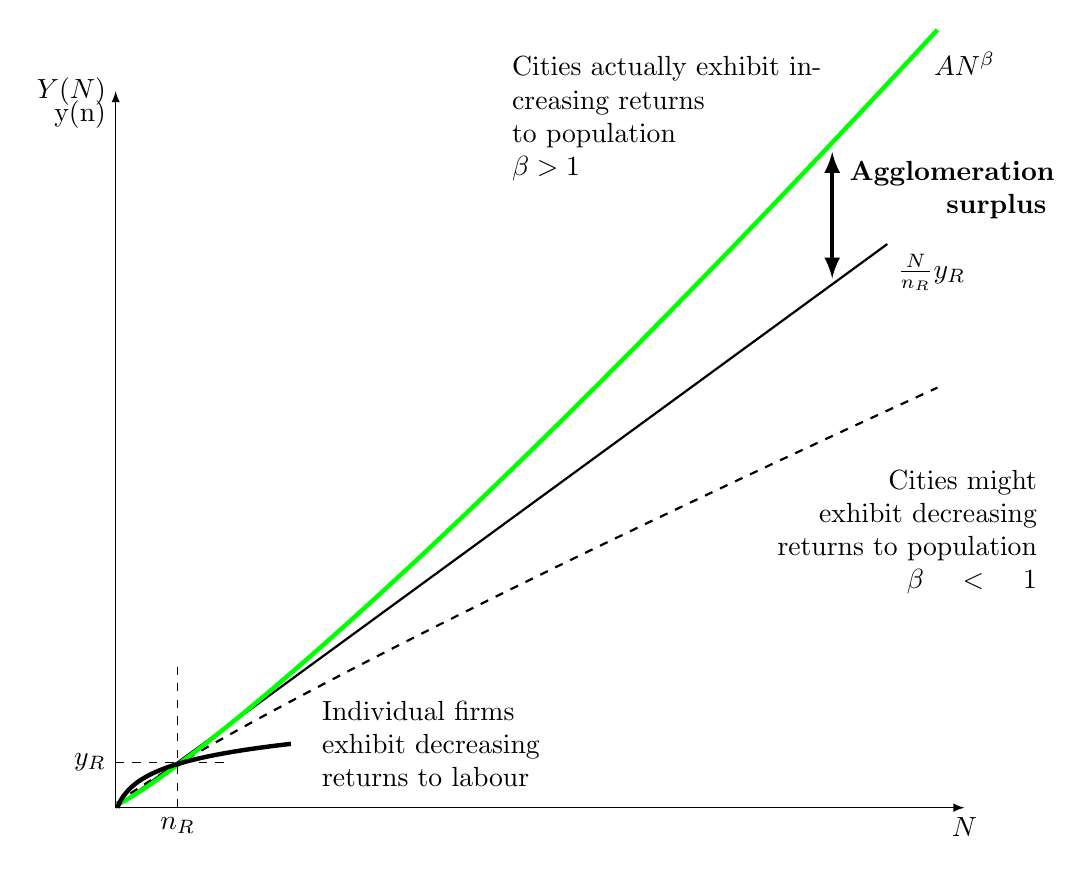
\begin{tikzpicture}[scale=.7, my plot/.style={thick, smooth, samples=100, domain=0.1:2.2},
plot2/.style={thick, smooth, samples=100, domain=0.1:14.99},
                    my grid/.style={dashed,opacity=0.5, every node/.style={black,opacity=1}},
                    my axis/.style={latex-latex}]
 
 \draw[my axis] (0,13)node[left] {$Y(N)$} --(0,0)-- (15.4, 0) node[below] {$N$}; 
%creates the axis 
 \node at (0,13)[below left]{y(n)};
 
\coordinate (origin) at (0,0);
\def\x{0.45}
\def\y{2.1}
\def\b {$15/(2*ln(\y)+.05)$};
%\def\p{0.55} % define the x, y and p )(midpointvalues
%\draw[my plot] (0,0) plot (\x,{ln(\x)});  %Draws curve
%\draw[my plot] (0,0) plot ({\x-.08},{2.3+ln(\x)}); 
\coordinate (Uy) at (\y,{2*ln(\y)+.05});

% THREE SCALE POSSIBILITIES
\draw [thick, ](0,0)--(14, 10.22583)node[below right]{$\frac{N}{n_R}y_R$};   %diagonal line CRS
\draw[plot2, dashed] (0,0) plot ({\x-.08},{(\x)^0.9/1.5 }); %DRS
\draw[plot2, ultra thick, green] (0,0) plot ({\x-.08},{(\x/1.5)^1.15});%
\node at (15.4, 13.5){$AN^\beta$};

%  TEXT
\node at (13.8,12.5) [left, text width=4.5cm]{Cities actually exhibit increasing returns\\ to population\\ $\beta>1$};%IRS
\node at (13.5,5)[text width=4.5cm, align=right] {Cities might\\ exhibit decreasing \\returns to population \\ $\beta<1$};% DRS

% ARROW
\draw[latex-latex, ultra thick] (13, 11.9)--(13, 9.6);
\node at (15.1, 11.2)[ text width=2.5cm, align=right]{\textbf{Agglomeration\\ surplus}};
%\draw[latex-latex] (13, 8.4)--(13, 9.5)node [below right, text width=1.5cm]{\textbf{$\pi$}};

\begin{scope}[ yscale=.75,xscale=1.5]% shift={(1.9,0)} ,
	\coordinate (Uy) at (\y, {2.3+ln(\y)});
  \draw[my plot,ultra thick] (0,0) plot ({\x-.08},{1.15+ln(\x)/2})node[right=.25cm, text width=3.9cm]{Individual firms\\ exhibit decreasing\\ returns to labour}; % production function for generic ferm
	\draw[dashed](.75, 0)node[below]{$n_R$} --(.75, 3.4);
    \draw[dashed](0,  1.1)node[left]{$y_R$} --(1.4,  1.1);
\end{scope}
%
%
%\begin{scope}[shift={(1.9,0)}]
%
% \def\x{0.45}\def\y{2}\def\p{0.55} % define the x, y and p )(midpointvalues
%\draw[my plot] (0,0) plot (\x,{ln(\x)});  %Draws curve
%
%\coordinate (start plot) at (0.6,{ln(0.16)}); % domain start
%\coordinate (end plot) at (10,10); % domain end
%%\draw[my axis] ([shift={(-0.5cm,0.5cm)}]start plot |- end plot) node[left] {$Y(\cdot)$} |- node[coordinate](origin){} ([shift={(0.5cm,-0.5cm)}]start plot -| end plot) node[below] {$L$}; %creates the axis a little 
%
%\coordinate (Ux) at (\x,{ln(\x)}); % set the u(x) coordinate on the curve. Not used
%\coordinate (Uy) at (\y,{ln(\y)}); % set the u(y) coordinate on the curve
%
%\draw [](origin)--(Uy)  ; 
%
%\draw[my grid] (Uy) |- node[below]{$L*$} (origin) |- node[left]{$Y^*$} cycle;%below from on curve, the 
%
%\end{scope}

\end{tikzpicture}

    \caption{While each individual firm exhibits decreasing returns to scale, the city as a whole exhibits increasing returns to scale, and thus produces an agglomeration surplus, $A(N^\beta)-\frac{N}{n}Y_F$.}
    \label{fig:Agglomeration-surplus}
\end{figure}

We need to distinguish the parameters of production functions for rural and urban firms and for the city as a whole. We assume that  rural and  urban firms use the same Cobb-Douglas technology $Y=A_FK^{\alpha_F}L^{\beta_F}$. The difference is that the urban firm enjoy a  multiplicative agglomeration externalize $N^\gamma$ which we assume is negligible for the rural firm and omit. $Y=A_FN^\gamma  K^{\alpha_F}L^{\beta_F}$.

In addition, there is an aggregate production function for the city from the scaling literature which we write $Y=AN^\beta$. We omit the subscript $C$ for city from  the aggregate production function.    

\subsection{TODO}


WHERE IS A?: param prefactor:  a  calculated initial value. Multiplier for e, called A. and empirical values form range in LOBO MOVE TO A

THINK ABOUT WHAT IT MEANS TO SAVE A SHARE OF NET RENTS IF ALL THOSE RENTS CAN BE PAID IN HOUSING RENT. CHECK IT'S DOCUMENTED
    %:param savings_rate: The share of the subsistence wage and net 
    % rent a worker can save in each time step, with undifferentiated labour 
    % and a uniform savings rate. SAME? TODO FIX


THINK ABOUT PREMIUM - ONLY BANK?
%     :param r_premium_person: Person's desired return over and above 
%     alternative investments.
%     :param r_premium_bank: Bank's desired return over and above 
%     alternative investments

\subsection{Parameter values}\label{sec-param-values}

\subsubsection{City}
\begin{description}
\item [density] workers per lot, maybe 100 initially, Combined with the city extent, $f$, this gives suburban population. % A high value reduces the computation time by reducing the number of cells, but it means we have a representative agent in  each cell. 
Notice we can set density individually for each cell in the grid, so density is really a vector variable.  % Also explore a density of 1 with a higher seed population.
\item [seed population] $P_0=0$. % An initial population at the center that anchors the population. % We need to seed it with an initial core urban Cities aren't unseeded. Zero initially, adjustable to get reasonable behaviour or to explore additional factors such as a service population or a retired population. 
\item [baseline population]  $N_0=\mathrm{density} * f_0 * f_0 + P_0$ 
\begin{lstlisting}
 self.baseline_population = density*width*height + self.seed_population
\end{lstlisting}
\item [initial wage premium ratio] $p_0\in\{0.04,0.2,.30\}$ (empirical range from various sources). The percentage by which urban wages exceed rural wages 
\item [worker share of urban agglomeration surplus] 0.72 or 0.8 $\lambda=\beta_F$ (Workers are getting the same share of the surplus and they do of output with no agglomeration effects.)
\item [urban agglomeration coefficient $\beta$ = 1.12] for the city: elasticity of urban output with respect to population (empirical)

\item [scaling adjustment factor] $z\in[0,1]$ Begin with z=0.5. Scaling adjustment for calculating the number of new entrants. 

\item [equilibrium cost of transportation] $c = \omega/f$. Constant.
\item [property tax rate annually. $\tau=0.04$]
\item [subsistence wage] $\psi$ = \$40,000. %  that is within range of reasonable subsistence wage in Canada for after-tax income. Try also lower values.
\item [workforce of a standard rural firm] $n=100$. This is also the initial value for urban firms.

\item[a: housing services share] Share of subsistence wage going to housing 
% services, a.


\item[b: maintenance share  of housing services ] Share of housing services going to maintenance.
\end{description}


\subsubsection{Land}
\begin{description}
\item[distance from center] 
\end{description}

\subsubsection{Person}
\begin{description}
\item[subjective discount rate] set $\mathrm{delta} = \mathrm{r_prime}$
\item[working period] age or working period out of the total number of working periods. People are initialized with a random working period between 0 and the number of working period (40).
\end{description}

\subsubsection{Firm}
\begin{description}
\item [initial workforce of a standard urban firm] $n_0=n$.  The urban firm workforce will evolve over time: $n_{Ut}$. 

\item [price of output] = 1. (If you wanted to be able to vary this, you would put a price parameter in front the % of marginal products. 
\gls{marginal product of labour}. %pMPL)

\item [firm cost of capital] $r = 0.05$ or 5\%.

\item [initial wage premium ]  \[\omega_0 = p \psi\] where $p$ is the wage premium ratio.

\item  [$\mathbf{\alpha_F}$] = 0.18 (typically 0.2 in macro models, but empirically values are lower, and lower values leave room for agglomeration effects),  for a single firm with a production function $Y_{Fi}=A_F K_i^{\alpha_F }L^{\beta_F}_i$ (empirical range =)\footnote{``In the U.S. from 1948-1995 the capital elasticity bounds were 0.18-0.33, and rose to 0.21-0.39 in 1995-2018.'' Dietrich Vollrath, (2021) The Elasticity of Aggregate Output with Respect to Capital and Labor. They also found that the capital elasticity in the private business sector is 0.09-0.28 from 1948-1995, and 0.16-0.33 from 1995-2018, and it is lower if intellectual capital is excluded.}

\item  [$\mathbf{\beta_F}$] = 0.72 (typically 0.8 in macro models, but empirically values are lower, and lower values leave room for agglomeration effects). Also called the elasticity of output with respect to labour for a single firm. (empirical)\footnote{Douglas  obtained a result for the exponent of labour of 0.75—which was subsequently confirmed by the National Bureau of Economic Research to be 0.741. Lower values  are associated with stronger decreasing returns to scale for the firm in our model.} 



\item [wage adjustment coefficient for new workers ] $adj^{new}_\omega=.5$

\item [wage adjustment coefficient for existing workers] $adj^{existing}_\omega=.5$
\end{description}


\subsubsection{Bank} % and mortgage parameters
\begin{description}
\item [mortgage period]  mortgage\_period (T)
\item [cost of capital for the bank] r\_prime. The bank's interest rate, $r$, is just the bank rate (r\_prime) set by the Bank of Canada.  
\item [r\_margin = 2\%] The bank's required markup on funds when it lends.  
\item [r\_target] reference rate that the bank demands on loans on 
$ r^{target}= r^{prime} +r^{margin}$ ? 





\item[lending rate/borrowing rate $r_i$]  
\[r_i=r^{prime} + r^{target} + \mathrm{individual\_wealth\_adjustment}\]



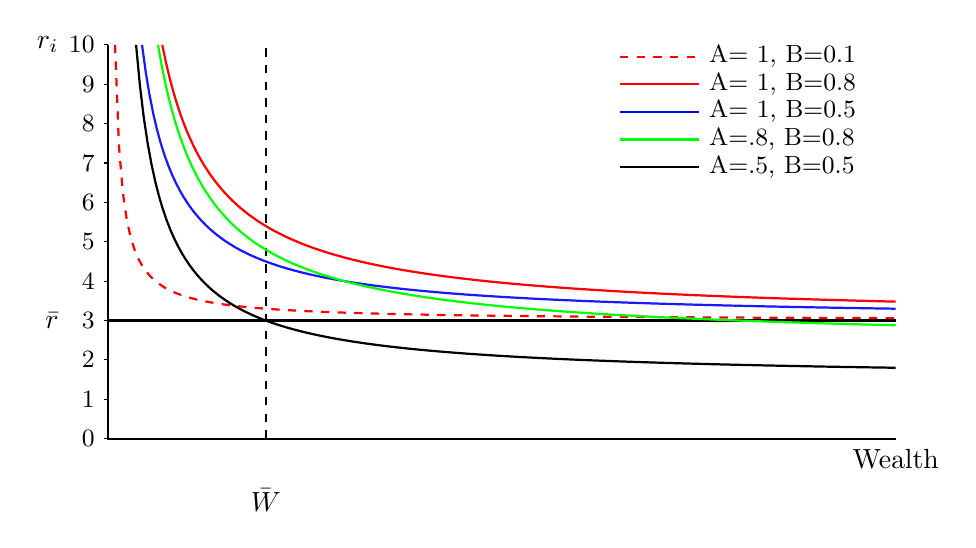
\begin{tikzpicture}[scale=.5]
%\def\bndmax{5}        %https://tex.stackexchange.com/questions/68462/filling-a-complex-region-with-tikz
%\def\bndmin{0.2}
\def \Y {10}  % height of y axis pecent
\def \W {20}  % length  of x axis
\def \Wbar {4} % jmeam wealth
\def \omega {3} % N.B.:  this is r bar

%Equation   \[ r_i = (A + .5 \frac{\bar{W}}{W_i})\omega\]
\def \Wmin{.63}  %This sets the lower limit fo the 
\def \Wmin{(\B*\Wbar)/(\Y/\omega-\A)} %function to keep in in bounds
	
\tikzset{func/.style={thick}}	

\draw [thick] (0,\Y)node[left=.5cm]{$r_i$} -- (0,0)--(\W,0)node[below]{Wealth};  	% Axes
\draw [thick] (0,\omega)node[left=.5cm]{$\bar r$} -- (\W,\omega);  	% Axes
\draw [thick,dashed] ( \Wbar,0)node[below=.5cm]{$\bar{W}$} -- (\Wbar,\Y);  	% Axes

\foreach \yi in {0,...,\Y} \draw (0,\yi)--(-.1,\yi)node[left]{\small$\yi$};

%     ORANGE
% \def \A {1} \def \B {.8}
% \draw[func,domain=\Wmin:\W, orange] plot [samples=200] (\x,{(\A/\x+\B*\X/\Wbar/\x)*\omega});
% \def \A {1} \def \B {.1}
% \draw[func,domain=\Wmin:\W, orange, dashed] plot [samples=200] (\x,{(\A+\B*\X/\Wbar/\x)*\omega});

%     RED
\def \A {1} \def \B {.8}
\draw[func,domain=\Wmin:\W, red] plot [samples=200] (\x,{(\A+\B*\Wbar/\x)*\omega});
\def \A {1} \def \B {.1}
\draw[func,domain=\Wmin:\W, red, dashed] plot [samples=200] (\x,{(\A+\B*\Wbar/\x)*\omega});

%.    BLUE
\def \A {1} \def \B {.5}
\draw[func,domain=\Wmin:\W, blue!90] plot [samples=200] (\x,{(\A+\B*\Wbar/\x)*\omega});
%     GREEN
\def \A {.8} \def \B {.8}
\draw[func,domain=\Wmin:\W, green] plot [samples=200] (\x,{(\A+\B*\Wbar/\x)*\omega});
%.    BLACK
\def \A {.5} \def \B {.5}
\draw[func,domain=\Wmin:\W, black] plot [samples=200] (\x,{(\A+\B*\Wbar/\x)*\omega});


\draw [red,  thick](13, 9)--(15,9)node [right, black] {\small A=\ 1,\ B=0.8};
\draw [red,  thick, dashed](13, 9.7)--(15,9.7)node [right, black] {\small A=\ 1,\ B=0.1};
\draw [blue,  thick](13, 8.3)--(15,8.3)node [right, black] {\small A=\ 1,\ B=0.5};
\draw [green, thick](13, 7.6)--(15,7.6)node [right, black] {\small A=.8, B=0.8};
\draw [black, thick](13, 6.9)--(15,6.9)node [right, black] {\small A=.5, B=0.5};
\end{tikzpicture}


\label{fig-capital-cost}

\item [{ability to carry a mortgage}] the share of income that can be used to cover mortgage interest. (rule of thumb: don't spend more than 25\% or 30\% we use 0.28.)
\item [maximum mortgage share of price] parameter in calculation of $m_i$. Specific to the functional form used. Set at 0.9. Based on stylized facts from the literature.  No empirical estimates are available.
\item[wealth sensitivity] of maximum mortgage share of price. This is a parameter in the calculation of $m_i$. It is specific to functional form used. Set at 0.1. The choice of a function is based on stylized facts from the literature.  No empirical estimates are available. Used in Equation~\ref{eqn-wealth-based-mortgage}.
\end{description}

DONE TO HERE.

\subsubsection{Realtor}


\subsection{TO ADD. Mostly definitions}

\subsubsection{locational rent}  $\omega-cd$ 

\subsubsection{warranted market rent} $\mathcal{R}_W=\omega-cd +a\psi$

The amount needed to fully pay housing costs and locational rent. This will include taxes and maintenance. Use  $\mathcal{R}_W$ as the initial rent cost for tenants,  $\mathcal{R}_{W0}$.

\subsubsection{warranted market price}   $P_W=\frac{\mathcal{R}_W }{r}$,  

This is the present discounted value of the warranted rents.  Use as initial market price.  (We anchor our housing price expectations in warranted rents, which, based on the literature can reasonably be seen as an equilibrium or attractor towards which prices will evolve. )

\subsubsection{Annual property taxation}
\[\mathcal{T} = \tau  \mathcal{P}_{M, t-1}\]

\subsubsection{Annual maintenance}
\[\mathcal{O}=   ba\psi \]

%%%%%%%%%%%%%%%%%%%%%%%%
 {\color{blue}
\subsubsection{initial \gls{market rent}} 
$\mathcal{R}_{M, 0}= \mathcal{R}_W$ 


This is what agents actually pay.\footnote{The market rent can in principle differ from the economically warranted rent as individual investors make decisions about rents and setting rents based on their own expectations, which include a wide range of factors. To simplify the model, we assume that the market rent equals the warranted rent. We are in effect imposing a long-term equilibrium value rather than modeling the adjustment process.} 


\subsubsection{Net rent for investors} {\color{green}}
\[\mathcal{R}_N = \mathcal{R}_W - \mathcal{O} - \mathcal{T}= \omega - {dc} + a\psi(1-b) -\tau  \mathcal{P}_{M, t-1}\]

The \gls{net rent} is the warranted rent net of costs. Homes must be maintained and taxes paid, so an investor would receive, not the total warranted rent, but the net rent after expenses,
}


\subsection{Initial values for endogenous variables} \label{sec-init-value-list}

These are \textbf{initial values} that we calculate based on the parameters above. These initial values provide  a starting point consistent with the production theory that we apply. They will be adjusted as the model iterates.  Some, like "Output for a typical rural firm", are simply intermediate variables used in further calculations.% that have to be chosen because they are used in calculating other values are:

\subsubsection{City}
\begin{description}

\item[number of urban firms] $F_0=\frac{N_0}{n_0}$.****

\item[elasticity of urban output with respect to population.] $\gamma$. Combining the two marginal productivity conditions, 
\begin{align}
\frac{n\psi}{\beta_F}  &= \frac{n(\psi+\omega)}{N^\gamma \beta_F}  \\
N^\gamma &= (1+\omega)/\psi)\\
\gamma &= \frac{log(1+p)}{log(N)}
\end{align}

\item [agglomeration surplus $\mathcal{S}$] We define the agglomeration surplus as the difference between the output produced by  the city with population N and a set of $N/n$ standardized rural firms each with a labour force $n$. 
\[\mathcal{S_0}=A^U N^\beta-F_0Y_R \] 
This is illustrated in Figure~\ref{fig:Agglomeration-surplus}

The surplus can also be expressed in terms of the wage premium and the workers' share of the surplus:
\[\mathcal{S_0}=N\omega_0/\lambda=\frac{N\omega_0}{\beta_F}\] 
The logic is that the wage premium is the worker's share of the urban surplus. We have assumed that $\lambda=\beta$ as a convenience but we could 
The logic is that the wage premium is the worker's share of the urban surplus. 

\item[urban scale coefficient $A_C$] Combining the two expressions for $\mathcal{S}$
\begin{align*}
 AN^\beta-\frac{N}{n}Y_F    &=\frac{N\omega}{\beta_F}\\ 
 AN^\beta   &=\frac{N\omega}{\beta_F} + \frac{N}{n}Y_F \\
 AN^\beta   &=\frac{N\omega}{\beta_F} + \frac{N}{n}\frac{n*\psi}{\beta_F}\\
AN^{\beta-1}   &=\frac{\omega+\psi}{\beta_F}\\ 
  A_C&=\frac{\omega+\psi}{\beta_FN^{\beta-1}}
\end{align*}
\textbf{NOTE: A is scale independent and all of the population agglomeration effects, which are confined to $N^\gamma$.}\footnote{We have assumed that $\lambda=\beta_F$ as a convenience but we could say $\lambda=zork*\beta_F$, making $A=\frac{\omega/zork +\psi}{\beta_FN^{\beta-1}}$ }
\end{description}


    \subsubsection{Land}
\begin{description}
\item[property taxes]
\begin{align*}
\mathcal{T} &= \text{mill rate} \times \frac{\mathcal{R}_W}{r} \\
&= \tau \times \frac{\omega_t- {dc} + a\psi.}{r}
\end{align*}


\end{description}

    \subsubsection{Person}
\begin{description}
\item [savings] $age_i*savings\_rate*\psi$


\item[personal wealth] $W_{i0}= savings + warranted\_price $
\item[average wealth] $\bar W_{0}= \sum_i W_i$
\item[Subjective discounting] The discount factor gives the present value of one dollar received at a particular point in the future, given the date of receipt and the discount rate.
% growth rate= rt
% growth factor =($1+r)^t$
% discount rate= r
% discount factor = $1/(1+r)^t$   
\begin{lstlisting}
def get_discount_factor(self):
    """
    The discount factor gives the present value of one dollar received at particular point in the future, given the date of receipt and the discount rate.
    Delta is the subjective individual discount rate for agent
    after one year. This will be close to the prime interest rate, r_i.
    """    
    delta = self.r_prime
    delta_period_1 = 1 / (1 + delta) 
    delta_mortgage_period = delta_period_1**self.mortgage_period
    sum_delta = (1 - delta_mortgage_period)/delta
    return sum_delta
\end{lstlisting}
% #   sum_delta = delta_mortgage_period * (1 - delta_mortgage_period) # Old
Delta could also depend on wealth. For example,  use the bank rate, which is the rational rate but people who are poor typically have higher rates.  It would not change as the central bank changes r-pirme
% delta could be wealth based typically higher for poor.

% sum\_delta is sum of the infinite series minus discounted infinite series after mortgage\_period years
% Here, it is the present value of annual payments from one to mortgage\_period years e.g. of mortgage payments or rent received. 
% delta\_mortgage\_period was previously called   delta\_period\_T 
% # Note delta_mortgage_period is subtracted to subtract the long tail. 1/delta gives the PV of an infineite series of payments

\begin{lstlisting}
# A version with delta depending on wealth
wealth = self.wealth
delta =
\end{lstlisting}
% savings =(sum(0-age)((1+r)**age)*savings_rate*subsistence)


\end{description}

\subsubsection{Firm $Y_{F,i}=A_FK_i^\alpha n_i^{\beta_F}$}
We use the familiar Cobb-Douglas production function \cite{chiangFundamentalMethodsMathematical2002} to set relationships among variables that are consistent with basic neoclassical production theory. 
\begin{description}

\item[initial urban wage premium] = $\omega_0 = (wage\_premium\_ratio) * \psi = p*\psi $

\item[initial labour force for urban firms] $n_0=n_R$.initially try values similar to the rural firm size and vary it  %*****%may have implicagtions later for the notation
\item[Initial wage premium] $\omega_0=p_0*\phi$
\item[Initial wage] = $\omega_0=\omega_t +\psi =(1+p_0)\psi)$
%The wage  is set as the marginal product of labour for initialization of the model. 

\item[labour cost for typical rural firm] $L_R = n_R*\psi$. This is expressed as a money quantity: e.g., 100 workers*\$40,000/worker.  

% \item[Initial labour cost for typical urban firm] ]  $L_U = n_R(\psi+\omega_0)$.

\item[output for typical rural firm]  
\[Y_R=\frac{n_R*\psi}{\beta_F}\]
This is a constant for any initial values. Derived from the marginal productivity condition. See item~\ref{item-paramlist-firm-level} in the orange  block. The numerical calculation is done  for a firm with 100 workers and a marginal product of labour of $\psi$. I get \$20 million for those values. 


\item[initial output for an urban firm] 
\[Y_0^U=N_0^\gamma Y^R\]  
Taking the marginal product with respect to $n$, we get a useful fact that will allow us to tie down $\gamma$
\[Y_{U,0}=\frac{n*(\psi+\omega)}{\beta_F}\]

\item[capital for typical rural firm] (Derived from the marginal productivity condition.)
\[K_R=  \frac{\alpha_R Y_R }{r}\]
This is also a constant.
 
\item[initial capital for an urban firm] (Derived from the marginal productivity condition.)
\[K_{U,0}=  \frac{\alpha Y_{U,0} }{r}\]
This is also a constant.

\item[scale factor A for typical  firm] 
\[A_F= \frac{Y_R}{K_R^{\alpha} {n\psi}^{\beta_F}}\]
We will assume that this is a constant used for both rural and urban production functions. (The explicit function is a bit  messy but the numeric value is easily computed because we have $L_r=n_R\psi$, and have calculated $Y_F$, and  $K_F$). The prefactor.

\end{description}

\subsubsection{Bank}
\begin{description}
\item[mean initial wealth $\bar W$] $= \frac {a\psi}{r_prime}+savings_0$
\end{description}

\subsubsection{Realtor}
\begin{description}
\item[None] 
\end{description}


\textbf{NOTE: With the initial values calculated in this section $\omega$ is consistent with $N_0$.as a result, population should not grow. }





\section{Model execution}
Variables that are recalculated in each step.\footnote{\begin{itemize}
    \item Variables have to have a time subscript. 
    \item We also distinguish the urban firm from the basic rural firm.  Only the urban firm changes its behaviour.  I use a subscript $_U$. 
    \item I omit the subscript for $n_t$ because only the urban firm changes its workforce size.
\end{itemize} }


\subsection{City}
\subsubsection{Wage premium ratio}

$p_t= \frac{\omega_t}{\psi_t}$ 


    \subsection{Land}
\subsubsection{Warranted price} The value of housing services including locational services. (Copied from the initial value calculation.)
\begin{lstlisting}
@property
def warranted_price(self):
    omega = self.model.firm.wage_premium # FIXED
    psi   = self.model.subsistence_wage
    a     = self.model.housing_services_share
    c     = self.model.transport_cost_per_dist # RENAME
    d     = self.distance_from_center
    r     = self.model.r_prime # CHECK name
  
    return (omega -c*d + a*psi)/r
\end{lstlisting}

\subsubsection{Maintenance costs for T} The discounted value (sum\_delta) of maintenance cost (b) on  physical housing ($a\psi$) over the mortgage period (T). This may be used in computing bids.
\begin{lstlisting}
def get_maintenance(self):
    """Maintenance share of property service (a*b*psi summed over mortgage period and discounted, like property tax)
    """
    a   = self.housing_services_share
    b   = self.maintenance_share
    psi = self.subsistence_wage
    sum_delta = self.sum_delta # CALCULATE PER PERSON
    return (a * b * psi) * sum_delta  
\end{lstlisting}

\subsubsection{Property tax rate for  T}
are imposed on the  warranted price (i.e., the value of the housing services) from the period before. They  are discounted value (sum\_delta)  over the mortgage period (T). This may be used in computing bids. A buyer assumes they are constant and paid at the end of each year of ownership during the mortgage period.
\begin{lstlisting}
    def get_tax(self):
        tau   = self.model.property_tax_annually
        omega = self.model.firm.wage_premium 
        psi   = self.model.subsistence_wage
        a     = self.model.housing_services_share
        c     = self.model.transport_cost_per_dist
        d     = self.distance_from_center
        sum_delta = self.model.sum_delta # TODO - make individual  - this would have to be average discounting - THIS TAKE SUM DELTA OUT - AND PUT WITH LARGER CALCULATION.. - CACLULATE FOR A PERSON/PROPERTY COMBINATION.
        return tau * (omega - c*d + a*psi) * sum_delta
\end{lstlisting}

\subsection{Person}
Does sum\_delta go here in person, or above the land (property ) calculations?  

\subsection{Firm}

\subsubsection{number of firms} $F_{t}=\frac{N_{t-1}}{n^{target}_{t-1}}$. Firm formation uses current variables to set number of firms for the next period 

\subsubsection{actual urban firms' employment} 
$n_t^{actual}= \frac{N_t}{F_t} $. Available workers are divided among existing firms.   


\textbf{actual urban firms' capital} in period t should be based on planned output rather than the labour available in the period, so we begin with the marginal productivity of labour equation, \[\omega_{t}+\psi = \frac{\beta_{F}Y^{target}_{t-1}}{n_{t-1}^{target}}\]
which gives us 


\textbf{urban firms' actual marginal product of labour}
\[MPL_{t} = \frac{\beta_{F}Y^{actual}_{U,t}}{n_t^{actual}}\] \noindent Firms observe their output, Yt and find  MPL= that they want to set equal to the wage. Al the values have been determined in the previous  and $n^{actual}_t$ is calculated using values from the  previous period, we get

\textbf{urban firms' output} by solving the above for Y
\[Y_{U,t}=  n_t^{actual}\frac{\omega+\psi}{\beta_{F}} \] 
This is used to calculate target employment.
% \item[(urban firms' capital)] (May not be needed)
% \[ K_{U,t}= \frac{\alpha}{\beta} \frac{n_{t-1}(\omega_{t-1}+\phi)}{r}\]


{\color{red}
\subsubsection{urban firms' target employment for $t+1$} Firms examine their own output and marginal product of labour, all calculated with values determined in the previous period. Following the  optimality rule, MPL=wage and MPK-r, they compute a target value for $n$ and $K$
\[ n^{target}_{t+1}= \frac{\beta Y_{t}}{\omega_t + \phi} \]



\subsubsection{aggregate urban labour demand of existing firms $N_{F,t+1}^{target}$} 

\[N_{F,t+1}^{target} = \frac{n^{target}_{t+1}}{n^{actual}_{t}} N_t\].   
This makes sense because Y is produced with the previous year's target assuming  $\gamma$ was constant but  $\gamma$ could have risen. (This should be the same result as  multiplying $n^{target}_{t+1} \times F_{t} $)



\subsubsection{New entrant labour demand,  $n\Delta F$} Firms enter when $MPL > wage$, which with existing technology permits profit making. New firms would set the same target employment as existing firms. 
\[n\Delta F =Z\frac{MPL_t-\omega_t -\psi}{\omega_t +\psi}F n^{target}_{t+1}\]
This makes sense because the number of entrants as a fraction of the existing number of entrants should be larger when the profit margin is larger. New firms would set the same target employment as existing firms and 

\subsubsection{Aggregate urban labour demand of existing firms $N_{Total,t+1}^{target}$} 
\[N_{Total,t+1}^{target}= N_{F,t+1}^{target}+n\Delta F\]

\subsubsection{Number of firm adjustment} 
\[F_{t+1}=\frac{N_{Total,t+1}^{target}}{n^{target}_{F,t+1}}\] 
This adjusts over time, keeping the firm labour force near the optimal level. 
{
\color{blue}
    \subsubsection{Wage adjustment for NEW workers} 
Firms want to increase output so they bid for new workers
\[wage_t^{new}= (1-adj_\omega)\omega_{t-1} + adj_\omega MPL_{t-1}  +\psi\] 

\subsubsection{Wage adjustment for EXISTING workers }
Existing workers demand catchup increases
\[ wage_t^{existing}= (1-adj_{exist})*\omega_{t-2} + adj_{exist}* wage_{t-1}^{new}  +\psi\]
Do we have to worry about workers switching firms? Would switchers get the full  bid new workers get? 
}
}
\textbf{wage adjustment factor} This is the fraction by which desired labour exceeds actual labour
\[\nu_t =\frac{N^{target}_{t+1}-N_{t}}{N_{t}}\]
or 
\[\nu_t =\frac{n^{target}_{t+1}-n_{t}}{n_{t}}\]



\subsubsection{Wage adjustment} 

\textbf{Wage calculation}
Firms make one decision faced with a market wage. They choose a target workforce. This is typical in \glspl{competitive market} where firms are price-takers. 


When \textbf{aggregate} firm labour demand exceeds N, wages rise at the city level

To get labour supply $N^s$ in terms of  $\omega$ we combine $N=f^2 *density$ and $f=2\omega/c$. 

So $\die{N^s}{omega}=4fden/c$ and \[\Delta \omega=  \frac{c}{4fden}\Delta N = \frac{c}{4fden}(N_{Total,t+1}^{target}-N_t)\]
This is the discrete wage adjustment that would attract the desired number of new workers, providing housing is available.\footnote{What happens is housing is not available? Maybe workers can't come to the city until the housing stock adjusts. Firms have labour shortages.  The wage stays high or may rise more. House prices will rise.} We can think of this as the wage demand of new workers.\footnote{What if only new workers get the new wage? This is interesting: firms will make excess profits. New firms will be attracted by excess profits but may not be able to get workers at the old wage!}

Should the adjustment occur in a single period?

It may be useful to put in an adjustment factor $adj \le 1$.
\[\omega_{t+1}=\omega_{t} + adj \Delta_t  \omega\]




% Common to think of the variations in local wages as variations around a mean, in this context - perfect labour market.
% We're using this number at the aggregate level, raise the market wage to a level that attracts that many. Divide available workers among the firms, then they want to raise the wage again. It's more transparent to do it at the aggregate level than at the firm level, but we still have the rising supply curve. A more detailed agent model could implement the hiring and wage adjustment mechanisms for firms directly, but the side effect of increased complication is it also can obscure the clarity of the rent results, our focus with this work. 
\begin{lstlisting}
# Firm step function updates wage, omega
def step(self):
    prefactor  = self.model.prefactor
    agglom     = self.model.agglomeration_ratio
    population = self.model.agglomeration_population
    wage_share = self.model.wage_share  
    wage_premium = wage_share * (agglom-1) * prefactor * population**agglom # omega # ****** 
    self.wage = wage_premium + self.model.psi
    # k thought # self.wage_premium = (wage_share * prefactor * population**agglom)/ population # omega    
    # note surplus is: (beta - 1) * (prefactor * population**agglom)
\end{lstlisting}

Where wage share is a parameter input to the model.


\subsection{Bank}\label{Parameters_for_Mortgages}


\section{Bidding}


\subsection{TODO Maximum bid price}

Agents compute their maximum bid, and the negotiation process adjusts downwards as appropriate REF.

\begin{eqnarray}
P_B^{max} & \le    \frac{\mathcal{R}_N}{(1-m)r^{target}-\delta \left(1 + \dot P_M^e - (1+r)m\right)} \label{eqn-bid-price} \end{eqnarray}

In banking with individual information on a land parcel and person.
\begin{lstlisting}
def get_max_bid_price(self, bidder, property):
    net_rent = property.get_net_rent()
    m        = bidder.get_max_mortgage()
    r        = self.model.sum_r # SAME AS SUM_R? RENAME?
    r_target = r_prime + agents_premium # FIX
    delta    = self.model.sum_delta # SAME AS SUM_DELTA? RENAME?
    P_dot    = GET FROM THE CURVE FIT
    denominator = (1-m)*r_target - delta*(1 + P_dot  - (1+r)*m)
    return net_rent / denominator   
\end{lstlisting}

\textbf{TODO FIX - little m is the max someone qualifies for.. we also have a maximum amount. Need to reconcile those two approaches.}
 


\subsection{Realtor}


\newpage

\section{Relationships that constrain parameters }

Explaining relationships that constrain parameters if the model is near an equilibrium path: 

CONSTRAINTS DIRECTLY FROM RESEARCH ON THE URBAN WAGE PREMIUM
\begin{enumerate}
     \item  Empirically the urban wage premium  $\omega$ is some fraction $p$ of the non-urban wage $\psi$.   This implies that if we set the subsistence wage, The urban wage is $(1+p)\psi$ and $\omega= p*\Psi$.


CONSTRAINTS DIRECTLY FROM THE CORE URBAN MODEL
    \item From the urban model, the extent of the city is determined by transportation costs:   $\omega =c*width$.  Only two of these parameters can be set independently.

    \item From the urban model population is determined by area and density   $N=density* f^2$. we assume the city is symmetric  and we assume plots  of land are identical, so  - $area=f^2$. If there is a core (or seed) population it must be added.  
   
    \item From the urban model the urban wage is the subsistence wage plus the urban wage premium $\omega+\psi$ 

CONSTRAINTS DIRECTLY FROM THE AGGLOMERATION/SCALE MODEL
    \item From the scale literature the value of aggregate output is $Y=AN^\beta$ for the city. This establishes a relationship between urban GDP and population. We initially make population equal to the workforce. 

    \item Empirically, $\beta \approx 1.13$


CONSTRAINTS DIRECTLY FROM THE NEOCLASSICAL THEORY OF THE FIRM
    \item From neoclassical theory of the firm the competitive equilibrium wage is the  marginal product of labour in the firm.      This should hold both in the urban and rural economies. This implies       $ MPL^R=\psi$  and $ MPL^U=\omega+\psi $.

    Using a Cobb-Douglas production function, we can get explicit expressions for the marginal productivities of labour and capital. 

CONSTRAINTS DIRECTLY FROM THE COBB-DOUGLAS PRODUCTION FUNCTION
The firm production functions are 
\begin{align}
Y_R  &= \quad  A_FK^{\alpha_F}L^{\beta_F}\\
Y_{R, )} &= N^\gamma A_FK^{\alpha_F}L^{\beta_F}
\end{align}
We start with firm labour forces  being equal at $n$.

\item $\sum_X \alpha_X \le 1$ is required for diminishing returns to scale. 

% \item From the theory of the firm with a general production function, an increase in the price of one-factor  results in increasing factor proportions for other factors.  

\begin{quotation} \color{orange}
\subsubsection{Firm level production}   
(This is incorporated above.) We want the marginal product of labour in the rural economy at the firm level to be at least close to \$40,000.  We can create a generic rural firm and then consider an urban firm with agglomeration effects to get the parameters we need. 

Firm employment $L$ is small relative to  urban employment {N}. Assume it is 100 workers. 

Assume that the rural production function is 
\[ Y_{iF}^R=A_{F} K^{\alpha_F} L_F^{\beta_F} \]
where  $L_F=n*\psi$, $\alpha_F=0.18 $,  and $\beta_F=0.76$.notice that the MPL is the partial derivative with respect to $n$ and not L. 
\footnote{These values give us diminishing marginal product at the firm level. If we require product exhaustion we have factor shares of  0.8 and 0.2.The tricky point is that factor share are 
 $\frac{\alpha}{\alpha + \beta}$ and $\frac{\beta}{\alpha + \beta}$
(*If not there is surplus profit  which we will ignore.)}   
The marginal products pf labour and capital are 
\[MPL=n*\beta_F Y_F/L_F=\$40,000\] and\[\ MPK=\alpha_F Y_F/K_F =0.05\]
From the first, 

\[Y_F=\frac{n*\psi}{\beta_F}=\frac{100*\$40,000}{0.72}=\$5,555,556\]
This is firm revenue. From the MPK, 

\[K_F=  \frac{\alpha_F Y_F }{r}=\frac{0.18 *\$5.5555\ million}{0.05} =\$20\ million = 1.039568 \]

We now have the capital, labour and output for a model firm with a marginal product of labour  equal to the subsistence wage we have chosen. We can calculate the \textbf{scale factor} 

\begin{equation}  
A_F= \frac{Y_F}{K^{\alpha_F} L^{\beta_F}}=\frac{5,555,000}{20,000,000^{\alpha_F} 100^{\beta_F}} = 1.039568 \label{eqn-AR}\end{equation} 
So $A_F$ can be computed using equation~\ref{eqn-AR} for any set of coefficients and firm size. Expanding the expression,

% \begin{equation}  %   arithmetic error here
% A_F 
% =\frac{\frac{n*\psi}{\beta_F}}{\frac{\alpha_F  \left(\frac{n*\psi}{\beta_F} \right)}{r}  L^{\beta_F}} 
% =\frac{\frac{n*\psi}{\beta_F}}{\frac{\alpha_F \frac{n*\psi}{\beta_F} }{r}  L^{\beta_F}} 
% =\frac{r}{\alpha_F  L^{\beta_F} }
% =6.944444e-08???? \label{eqn-AR2}\end{equation} 

Furthermore, we can compute the output for a city of size N if it consists of $N/n$ firms of this type. With a population of 10,000, for example,  there would have to be  100 firms and an output of \$555,555,600. 

 \subsubsection{The urban level of production}
 \textbf{This section now redundant and has been commented out}
% We now consider that this firm operates in the city and enjoys  urban agglomeration benefits. The value of the  marginal product of labour must rise to $\psi+\omega$. We to know  the urban wage premium that is consistent with the subsistence wage. Papageorgiou \cite{papageorgiouOccupationalMatchingCities2022} found a 4.1\% premium. D'costa and Overman   show that working in London is associated with a 35.5\% higher wage than working in a rural area. The comparable figures are
% 10.6\% for big cities and 8.3\% for small cities and an elasticity of wages with respect to city size of 1.6\%.. Estimates of the premium are lower  when they control of individual characteristics.   

% If the $ scale\ coefficient=1.12$, $=\omega$ would be $1.12*\psi$, or $4,800$. 

% This supports an urban wage premium of $\omega\$8,000$.

% We need to have a population size or a number of firms with a firm size. Assume the population is 10,000 and firms still have 100 workers. (All firms will have the same marginal product of labour in a competitive labour market, so size should not matter.)

% \[Y^U=A^R N^\gamma K^\alpha L^\beta = N^\gamma Y^R\]
% where $N^\gamma$ represents the agglomeration effect. The marginal product of labour is 
% \[MPL^u=\$44,800=N^\gamma \beta Y^R/L=N^\gamma *\$40,000\]
% so $N^\gamma= 1.2$ and $\gamma = \frac{log(1.12)}{log(10,000)} =.012$. 


% This value is consistent with an empirical  value for  the agglomeration exponent of $\beta =  1.012$. The value is much lower than empirical estimates. Furthermore, if we consider the same firm structure and a population of one , the value falls, which suggests that agglomeration effects are not scale-independent, but instead increase with urban size. $\beta$ may itself be a function of $N$.

% % A second interesting possible implication of our calculation is that only part of the agglomeration effect appears in wages. Urban rents  are large, but agglomeration effects are much larger.
\end{quotation}

\end{enumerate}



\footnote{Tørsløv et al \cite{torslovMissingProfitsNations2023} show that affiliates of foreign multinational firms are an order of magnitude more profitable than local firms in a number of low-tax countries. Leveraging this differential profitability, they estimate that 36\% of multinational profits are shifted to tax havens globally. US multinationals shift twice as much profit as other multinationals relative to the size of their foreign earnings.}


\textbf{appendix-05-agglomeration-model - REDUNDANT} %\renewcommand{\sfdefault}{phv}

\section{Initial values for  the agglomeration parameter}
A segment is now redundant and has been commented out

\vspace{5lines}

% {\Large  $Prefactor = 1506.712$ based on width=height=10 and density=100} and agglomeration\_coefficient= 1.2,
% We need to get the scales of the parameters and the population size roughly consistent.

% I assume the 10X10 grid is full. 

% \section{Computing the prefactor: details}
% We have set the subsistence\_wage to \$40,000.

% The urban wage premium is in the range of 13-20\%  Assume 20\% and we get \$8,000

% Under the neoclassical assumption  \$40,000 is the  marginal productivity of rural worker

% The urban production function is 
% \[Y=AN^\beta\]
% \[Y=prefactor*working\_population**scaling\_exponent\]

% where $working\_population = width*height*density$ 

% so 
% \[Y=prefactorA*(width*height*density)^{\beta}\]

% We have more conditions that this has to satisfy: The marginal product must be consistent with the urban wage and the distribution rule. The wage cannot add up to more than total output output. Workers cannot get 1.2Y/N, for example. With CRS they would get 0.8Y/N.    

% \subsection{approach one: from agglomeration surplus}
% \[urban\_wage= subsistence\_wage + wage\_share * agglomeration\_surlpus\]
% The \textbf{agglomeration surplus} is the excess relative to the CRS case when $\beta=1$:
% \[agglomeration\_surplus= A(N^{1.2} -N^1) \]
% The urban wage premium is then the share for each worker:
% \[\omega= wage\_share * \frac{agglomeration\_surlpus}{N}\]

% and this becomes
% \[\omega= wage\_share * A\left(\frac{N^{1.2}-N^1}{N}\right)=1 * A\left(N^{0.2}-1\right)\]

% To see what this looks like, consider a population of 10,000 when  wage\_share=1
% \[\omega= \$8,000 = A\left( 6.309-1 \right)\]

% {\Large So $A = 1506.712$ based on width=height=10 and density=100}  

% Smaller N makes A bigger

% % Say width=height=15 and density= 200:
% % \[\omega= \$8,000 = A\left(10000-1\right)\]

% \subsection{Approach 2: from Marginal product and subsistance wage}
% % We want the marginal product of labour in the rural economy at the firm level to be at least close to \$40,000.

% % Firm employment $L$ is small relative to  urban employment {N}.  We can create a generic rural firm and then consider an urban firm with agglomeration effects to get the parameters we need. 

% % Assume that the rural p[rooduction function is 
% % \[Y^R=A^R K^\alpha L^\beta\]
% % where $\alpha=0.2$  and $\beta=0.8$. The marginal products are 
% % \[MPL=\beta Y/L=\$40,000\] and\[\ MPK=\alpha Y/K =0.05\]
% % From the first, 

% % \[Y=\frac{L*\$40,000}{0.8}=\$5\ million\]

% % This is firm revenue. From the MPK, 

% % \[ \frac{0.2 \$5\ million}{0.05}=K =\$20\ million \]

% % We now have the capital, labour and output for a model firm with a marginal product of labour  equal to the subsistence wage we have chosen.

% % We now consider that this firm operates in the city and enjoys  urban agglomeration benefits.  If the scale coefficient=1.12$,$ $\omega$ would be as a first appr Say that the marginal product rises to \$48,000. This supports an urban wage premium of $\omega\$8,000$.

% % We need to have a population size or a number of firms with a firm size. Assume the population is 10,000 and firms have 100 workers. All firms will have the same marginal product of labour in a competitive labour market, so size should not matter. 

% % \[Y^U=A^R N^\gamma K^\alpha L^\beta = N^\gamma Y^R\]
% % with a marginal product of 
% % \[MPL^u=\$48,000=N^\gamma \beta Y^R/L=N^\gamma *\$40,000\]
% % so $N^\gamma=1.2$ and $\gamma = .019$. 


% This value is consistent with an empirical  value for $\beta$   1.02. The value is lower than empirical estimates. Furthermore, if we consider the same firm structure and a population of one million the value falls, which suggests that agglomeration effects are not scale-independent, but instead increase with urban size. $\beta$ may itself be a function of $N$.

% A second interesting possible implication of our calculation is that only part of the agglomeration effect appears in wages. Urban rents  are large, but agglomeration effects are much larger.


 

% %\[subsistance_wage= MPL(\beta=.= \]
 % bbbb{appendix-05-agglomeration model}



\begin{enumerate}
\item To start with a population of around 10,000, we begin with width = 10, height = 10 and \textbf{density} per unit of 100. 

\item If we arbitrarily assume an initial wage premium around 20\%, and wish to start near equilibrium, % bettencourt assumed aggomeration exponent is indepent)
we can select transportation costs. A transportation cost of 0.1  would give a distance of $\omega/.01$, which is huge. Could this be 1/10 of the starting wage premium $\omega_0$? It would then be \$800 per year, per unit distance and would give us height and width of 10. 
% (divide into omega) - we want to start close to equilibirum. omega/cost = width
\item We should have a wage premium of about \$8000 to be consistent with the subsistance wage. % since we are assuming the wage premium of around 20%. Total wage has to be subsistence wage + wage premium, think of an average rural subistance wage seems like 45K .. 

\item Your proposed prefactor was 0.2,  251. It should be very large, based on the above numbers and the consistency constraints. I get 1507 in appendix-05-agglomeration model

\item Teminology: Y=prefactor*N**scaling\_exponent

\end{enumerate}

\begin{lstlisting}
def __init__(self, width = 50, height = 1,  # ****
             transport_cost_per_dist  = 0.1,    # c   ****
             subsistence_wage         = 40000. # psi
             working_periods          = 20,     # in years ****
             savings_rate             = 0.2, ****
            #  initial_savings: if agents save anything before reaching working age
             init_wage_offer          = 10.,  #. Makes no sense  ****
             init_interest_rate       = 0.05,

             #AGGLOMERATION MODEL features  -20% wage premium over subsistence wage, Y=prefactor*N**scaling exponent
             prefactor                = 0.2, # 251., ??????  ****. should be very large. I get 1507 
             # Prefactor - should be much higher than YES scaling_factor           =   # this is A scaling_exponent         =  1.13 # this is beta in LOBO. ****
             agglomeration_ratio      = 1.2,  # beta, was 
             wage_share               = 1.0,  # of agglomer3ation benefits
             workers_share            = 0.8   # emponent? in Slae models?
             property_tax_annually    = 0.04, # tau, was c
             mortgage_period          = 5.0,  # T, in years
             housing_services_share   = 0.3,  # a
             maintenance_share        = 0.2,  # b
             r_prime                  = 0.05,
             r_premium                = 0.005, ****
            #  r_premium_bank = 0.00, # TODO: heterogenous discount rates and premiums
             ):
\end{lstlisting}

\subsection{Workers share}
The worker's of the surplus, $lambda$ It might be 0.8. It is used in...

NOTE: 0.8 is the value of beta in a Cobb-Douglas, corresponding to the wage-share in production. It is the value used in Lobo et al


\section{Older parameter value discussion}

\subsection{Price growth}
% """ Note agents forecasts are linear, but the population growth 
% is power law distributed. Thus the model is conservative and agents
% underestimates the the value of the urban center. Actuall effects  
% could be stronger. onsider alternative appraoches to forcasting value, risk, etc.#     What time frame do agents consider? Is their model linear?

\subsection{Time}
 The computational cycle is a year, so all time-dependent variables, such as wage, transportation cost, and interest rates, are specified for the yearly interval. The mortgage period is set arbitrarily 
 
\subsection{Wage premium} \label{section-wage-premium}

Hirsch Wage \cite{hirschUrbanWagePremium2019} observe that, ``Following Glaeser and Maré \cite{glaeserCitiesSkills2001},  a  large  empirical  literature  has  investigated differences in wages across labour markets of different sizes. The general finding of this literature is that a significant urban wage premium exists. and that this premium consists both of a level effect and a growth effect that arises as workers gain urban work experience.'' 

Almeida et al \cite{almeidaUrbanWagePremium2022} found for Brazil, that the female urban wage premium is on average 11.3\%, almost double the average male premium of 5.7\% and that higher in formal and informal jobs and across various agglomeration levels. The premium is larger in denser areas.

\subsection{Spillover effects} \label{section-spillover}

Spillover effects can be large. Irwin and Klenow  studied learning in chip production focusing  on the key issue of spillovers. They found learning rates of 10 to 27 per cent, averaging 20 per cent. They indicated that a good part of learning is internal, and that national spillovers were no greater than international spillovers. " \dots a firm learns three times as much from an additional unit of its own cumulative output as from another firm's cumulative output, regardless of the other firm's country of location. However, rest-of-world cumulative production is typically more than three times any given firm's cumulative production. This means that the absolute contribution of world cumulative production to each firm's experience outweighs the absolute contribution of its own cumulative production. In this sense, spillovers are substantial." (pp. 1217-1218).


\subsection{Property taxes}

mills

Each mill is expressed as  1/1,000 of the value as determine by assessment \footnote{By capitalizing the mill rate at 5\%  we see that each `mill' is worth about 2\% of the warranted rents. Assessments usually understate the market value considerably. Mill rates are commonly about 1.5 and differ between municipalities. ***MAYBE MOVE PARAM VALUES TO PARAM DISCUSSION}


\section{Transportation parameter values}
In the following sections we and present illustrative values for parameter values.


%==========================EXAMPLE=========================== https://www.kaggle.com/code/prateekmaj21/basic-financial-calculations-using-python/notebook
  
% def compound_interest(p,r,t):  %EXAMPLE
    
%     print('Amount: ', p)
%     print("Rate of Interest (Per Annum)", r)
%     print("Time (In Years): ",t)
    
%     a= p*((1+r/100)**t)
    
%     ci= a-p
%     print("Final Amount: ", a)
%     print("Compound Interest: ", ci)
 

\section{Transportation costs}
Transport costs have two parts:
1) fuel and vehicle costs per km
2) time costs per km

\subsection{Vehicle related costs}
Use one year as the wage period, converting transportation costs per km to annual cost for consideration in the household budget. Starting with the cost per km, calculate the cost per year:

\textbf{cost per km =$\textit{t}$}:. \$0.59   (from  Ontario data, 2021). sensitive to congestion, use of subways (\$5 /day?), 

 \textbf{work trips per year} 2 way * 5 days/week * 50 weeks work days = 500. [range: 450-550]

\textbf{cost per km-year} = work trips per year*cost per km

=\$0.59/km*500 trips/year  =  \$295/km year 



\subsection{Time costs}
\textbf{time per km}. range: 20km/hr -> 3min/km, 40km/hr -> (1.5min/km - 3min/ km)per trip 

(New York rush hour is much slower:  4-9km/hr ->6-15 min/km)

\textbf{time  per km-year} = work trips per year*time t per trip = 500* 3min  = 1500 min/km year = 25 hours= 3-3.5 days/km
 
\textbf{time cost per km-year} =  (days per km-year /work days/year)*wage premium per year  = 3/250 = 0.012 years/km year. ?

\textbf{money cost of time per km year} 

=time cost per km-year* wage(including subsistence) 

= 0.012 year* wage per year

\subsection{Total cost per km year of commuting for one agent}
\textbf{money cost of time per km year + \$295/km year * distance} \\
= (0.012 w+ \$295)/km year 
    \begin{quotation}
    \textbf{Example}
    To get a sense of the required wage if we have this annual cost structure, assume city\_extent $d^*$ is 30 km. At this point the transport cost is equal to the wage

\[(0.012 w+ \$295)/km year)*30 =  w\] 
\[.36w+ 8850=w\]
\[w=13828.12\]
        \begin{quotation}
        \textbf{PLAUSIBILITY CHECK}
This is plausible land rent, but does not include building rent. 
Capitalized at 5\% this house is worth \$ 276,562, a fairly cheap house 30 miles from city centre
        \end{quotation}
    \end{quotation}



\subsection{Value of transportation price to use in model}
\[ {c}=(0.012 w+ \$295)/km year \]



\section{Table of parameter values}

\renewcommand{\arraystretch}{1.5}
\begin{tabular}{rlrr}
Symbol         & Name                                 & Value      & Formula  \\ \hline
$a$ replace    & Share of $\psi$ for land and building &   0.3         & \\
$b$ replace    & Share of $\psi$ for maintenance       &   0.2         & \\
$tau$ replace  & Property tax rate &  e.g 1.6\% = 16 mills             & \\
$c$       & Transportation cost & \\
$T$       & Period & 5 years      \\
$r$       & Individual interest rate & 0.05 \\
$\omega$  & Locational rent & 0.012  \\
$\psi$    & Subsistence wage & 10000 \\
$a$       & Share of subsistence wage for land and building & 1.0 \\
$\tau$       & Tax share & \\

---       &  & \\
$m_i$          & Individual borrowing-ratio           & 0.75-0.85  & $M/P^{ask?}$ \\
$M^{max}_Yi$.  & Maximum mortgage based on income     &            & $\frac{0.28(\omega+w)}{r_i}$ \\
 $M^{max}_P$   & Maximum mortgage based on the price  &            & $0.8*P_0$ \\
$IS$           & Income share for housing debt        & 0.25-0.35  & Missing? \\
$\rho$         & Rent ratio                           &            & $\frac{\omega-tau*d_i}{P_0}$ \\
$\kappa $      & Operations ratio                     & 0.1-0.3    & e.g. $ 0.2\frac{\omega-tau*d_i}{P_0}$ \\
$\sigma$       & Tax ratio                            & 0.25-0.35  & e.g. $ 0.3\frac{\omega-tau*d_i}{P_0}$ \\
$\dot P $      & Price growth                         & []         & $\frac{P_t-P_{t-1}}{P_{t-1}}$\\
% $P^T_e$        & Expected price in T years            &            & $P_0(1+\dot P)^T$ \\ % *** WAS $P^e_T$ 
$r_i^\delta$   & Individual discount rate             &            & To assign \\
$\bar r$       & Prime interest rate                  &            & \\
$r_i$          & Individual borrowing-rate            &            & \\
$r^{target}$   & Target interest rate                 &            & $\bar r + margin$ \\
$\delta_i$     & Discount factor for T                &            & $\left(\frac{1}{1+r_i^\delta}\right)^T$ \\


\end{tabular}
\renewcommand{\arraystretch}{1.0}




discount rate vs discount factor

% delta(0)=1  delta (1)= 1/(1+r) 
\[\delta(t)=\left(\frac{1}{1+r}\right)^t\]
    $delta_T=  (1/(1+r))^T$   at T years
    eg r=.05  T=5  delta5 =  $(1/(1+.05))^5 = 0.7835262$
